% Basic Electronics Training
% Updated 1/24/2017

\chapter{Basic Electronics Training} \label{basic_electronics}
\section{Introduction}
The M:2:I lab has equipment that is suitable for a wide range of electrical work, diagnostic and repair.  The lab has a sectioned off area that is dust controlled and has work surfaces that is static controlled.  This creates a suitable work environment for working on a number of electrical projects.

The electrical area has work benches that is divided up to 3 stations.  Station 1 contains advanced diagnostic and soldering equipment and requires additional training beyond the scope of this section.  Station 2 and 3 has basic diagnostic soldering equipment and will be covered in this section.

Station 2 and 3 has the following equipment at each station.  In addition, these stations are suitable for the following activities.

\begin{itemize}
\item Soldering and de-soldering components
\begin{enumerate}
\item Through hole components
\item Surface mount components
\end{enumerate}
\item Lab bench power supply
\begin{itemize}
\item 0 - 30 VDC @ 3 amp controlled supply
\item power consumption logging
\end{itemize}
\item Waveform generation
\item Waveform measurement
\end{itemize}

It should be noted that the work bench is a Electro Static Discharge (ESD) safe and is designed to minimize ESD when used properly.  This requires that users are properly grounding themselves and using the wrist-straps that are attached to the bench.  An additional work mat is also at each station which is also ESD safe and helps protect the bench from soldering.

\begin{framed}
\begin{wrapfigure}{L}{0.14\linewidth}

\includegraphics[width=\linewidth]{images/important_icon.png}
\end{wrapfigure}
\ \\
Students working at the electronics stations must take care to not damage any of the mats.  No cutting is permitted at any time with these mats and care should be taken when soldering to prevent burning.
\end{framed}

\section{Hazards}
The following are possible hazards when working with any of the equipment in the electrical work bench area.  Please take note of these hazards and make sure you understand the possible dangers and the steps needed to reduce possible harm to yourself.

\begin{framed}
\begin{wrapfigure}{L}{0.15\linewidth}
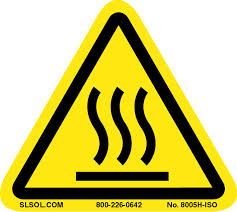
\includegraphics[width=\linewidth]{images/burn_hazard.jpg}
\end{wrapfigure}
\ \\
Burns are possible both from the soldering iron and heated materials during the soldering process. Always utilize the soldering iron stand and always look when reaching for the iron. Never solder with unsupported materials or over your body. Heated materials may fall from the connection and cause severe burns.
\end{framed}

\begin{framed}
\begin{wrapfigure}{L}{0.15\linewidth}
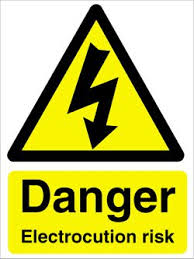
\includegraphics[width=\linewidth]{images/electrocution_hazard.jpg}
\end{wrapfigure}
\ \\
Electrocution is always a possibility when working with electronics. Keep liquids away from the workbench at all times. Always double check your electrical connections. Only energize the circuit when necessary and move the circuit as little as possible while energized. Proper use of the over-voltage and over-current controls can help to minimize any damage or injury caused by a short circuit condition.
\end{framed}
\ \\
\ \\
\begin{framed}
\begin{wrapfigure}{L}{0.16\linewidth}

\includegraphics[width=\linewidth]{images/fumes_hazard.jpg}
\end{wrapfigure}
\ \\
Hazardous fumes may result from the decomposition of solder, fluxes, cleaning agents and other soldering substances or from substances on the materials being soldered. Fumes released during soldering are generally within allowed exposure limits but care should be taken.  Proper use of the smoke extractor will minimize any possible effects from these fumes.
\end{framed}

\subsection{Chemicals}
Chemicals used while soldering, including lead, may cause skin or eye irritation or may be ingested. Gloves should be worn when dealing with any substance marked as hazardous and hands should always be washed after soldering or handling soldering materials.

\section{Electronics Equipment}
The following is additional information on each piece of equipment that you can find at both station 2 and 3.  Information on Station 1 can be found in the Advanced Training in Chapter 

\subsection{Weller WES51 Soldering Iron}
The Weller WES51 shown in Figure \ref{fig:wes51} is a standard soldering iron that has the following features:

\begin{itemize}
\item 50 watt pencil iron,
\item Replaceable tip sizes,
\item 350 to 850 degrees F,
\item Temperature stability +/- 10 degrees F,
\item Temperature accuracy +/- 10 degrees F.
\end{itemize}

\begin{figure}[ht]
\centering
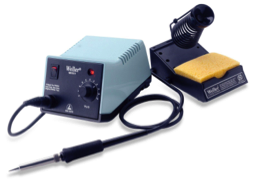
\includegraphics[width=2in]{images/wes51.png}
\caption{The Weller WES51 Soldering Iron}
\label{fig:wes51}
\end{figure}

The WES51 has the ability to have both different sizes and shapes of tips that can be used.  In general, the soldering iron is equipped with a fine conical tip.  This type of tip is suitable for light general purpose soldering and for some surface mount soldering.  The lab does have some some other sizes and shapes of tips available.  Please see a lab monitor or Matthew Nelson if you need a different tip.

\subsection{Rigol DP832 Programmable DC Power Supply}

The Rigol DP832 shown in Figure \ref{fig:dp832} is a programmable lab bench DC power supply.  It has the following features:

\begin{itemize}
\item Three adjustable outputs: 30V/3A, 30V/3A, 5V/3A,
\item Up to 195W total power,
\item Programmable over-voltage/over-current protection,
\item Programmable voltage waveform,
\item Voltage/Current/Power waveform display/logging.
\end{itemize}

\begin{figure}[ht]
\centering
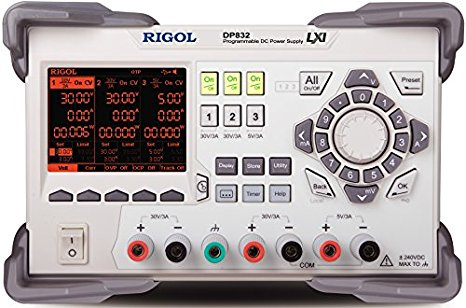
\includegraphics[width=2in]{images/dp832.jpg}
\caption{The Rigol DP832 DC Power Supply}
\label{fig:dp832}
\end{figure}

\subsection{Rigol DS1102E Digital Oscilloscope}
The Rigol DS1102E Digital Oscilloscope shown in Figure \ref{fig:ds1102e} is suitable for reading a number of waveforms for diagnostic purposes.  It has the following features:

\begin{itemize}
\item Two channel, 1 GSa/s maximum real-time sample rate,
\item 100 MHz bandwidth,
\item 10 Kpts memory depth,
\item Image and data export to USB drive.
\end{itemize}

\begin{figure}[ht]
\centering
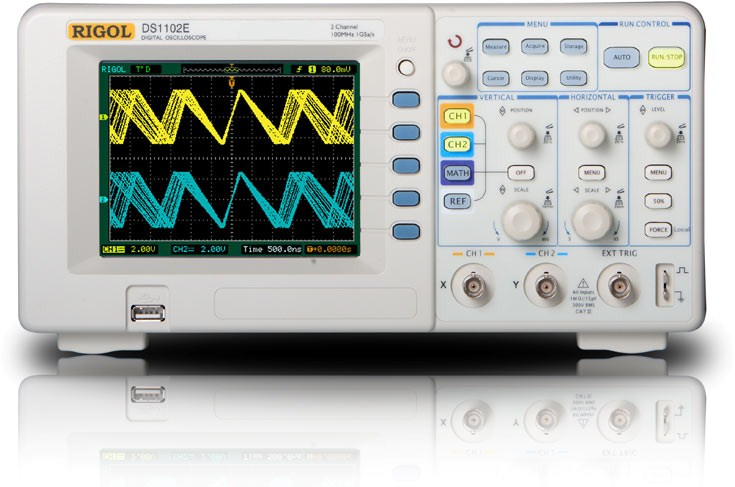
\includegraphics[width=2in]{images/DS1102E.jpg}
\caption{The Rigol DS1102E Digital Oscilloscope}
\label{fig:ds1102e}
\end{figure}

\subsection{Rigol DG1022A Arbitrary Waveform Generator}
The Rigol DG1022A shown in Figure \ref{fig:dg1022a} is a lab bench wave form generator that is able to generate a number of waveforms and frequencies for testing and diagnostics.  This generator has the following features:
\begin{itemize}
\item Two channel arbitrary waveform up to 25 MHz,
\item Modulation functions (AM, FM, PM, FSK, etc),
\item Frequency counter up to 200 MHz,
\item 100 MSa/s sample rate, 14 bit accuracy.
\end{itemize}

\begin{figure}[ht]
\centering
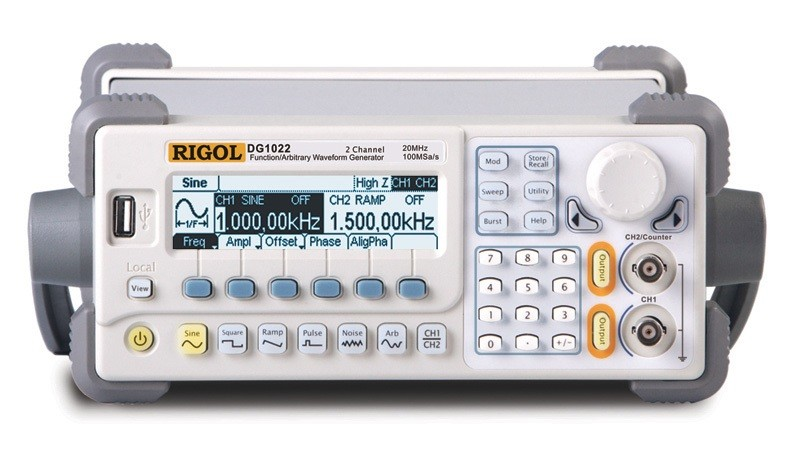
\includegraphics[width=2in]{images/dg1022a.jpg}
\caption{The Rigal DG1022A Waveform Generator}
\label{fig:dg1022a}
\end{figure}

\chapter{Electronics Procedures}
Student should be familiar with the general procedures for using the equipment at the electronics bench before using them.  The following procedures are there to provide guidance to students in using the equipment at the electronics workbench.  It is not a comprehensive guide but should help students in getting started with the equipment.  If at any time you have questions please see the M:2:I Program Coordinator.

\section{Soldering Procedures}
Soldering is a skill that does take some practice.  A good solder joint will provide both a good electrical connection and securely hold contact or pin to the printed circuit board.  A poor solder connection however can cause intermittent behavior in the circuit and can cause the circuit to fail.

The electronics lab has two types of solder, lead based and lead-free solder.  Lead-free solder is recommended for most projects, but in some cases, such as critical applications, it should not be used.  An interesting fact, the lead-free solder (Tin-Silver-Copper) was actually developed here at Iowa State University in the Ames Laboratory and with Sandia National Labs-Albuquerque.

\begin{framed}
\begin{wrapfigure}{L}{0.14\linewidth}

\includegraphics[width=\linewidth]{images/important_icon.png}
\end{wrapfigure}
\ \\
The use of leaded solder can be hazardous to the students health.  If leaded solder must be used, it should be handled with gloves and soldering should take place with a fume extractor in use.  Doing this will minimize the introduction of lead into the body which is toxic.
\end{framed}

\subsection{Soldering}

\begin{framed}
\begin{wrapfigure}{L}{0.15\textwidth}
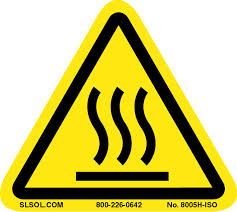
\includegraphics[width=.7in]{images/burn_hazard}
\end{wrapfigure}
\ \\
The tip on a soldering can reach temperatures of 400 C (750 F) and higher.  Always use caution when using a soldering iron and always be aware of both your surroundings and where the soldering iron is.  While most surfaces in the electronics area can handle short durations of heat, you can not.
\end{framed}

\begin{framed}
\begin{wrapfigure}{L}{0.15\textwidth}

\includegraphics[width=.7in]{images/fumes_hazard}
\end{wrapfigure}
\ \\
Fumes produced from soldering can be hazardous to your health with both leaded and lead free solder.  Fumes can irritate and cause harm to both your lungs and eyes.  You should always use one of the ventilation fans to pull the fumes away from you.
\end{framed}
Soldering involves heating up the \emph{pad} and the \emph{pin} to allow the solder to flow and on the part.  In most cases you \emph{do not} want to heat up the part itself.  In many cases doing so will result in damage to the part.  The key to soldering is apply even heat to the pad and allowing the solder to flow on the pad and pin.  A good solder joint will look like Figure \ref{fig:good_solder}.  The following steps should be followed to ensure good soldering techniques.

\begin{enumerate}
\item Ensure station has a brass sponge or a wetted sponge.
\item Set the iron to the correct temperature, when the LED is rapidly flashing the iron is at the set temperature
\item Clean the iron using the brass sponge or wet sponge
\item Tin the tip of the soldering iron
\item Heat the pad or joint and then apply solder to the pad or joint
\item Once the solder is melting apply enough to ensure a good connection
\item Remove the iron once done with the solder
\item Clean the tip as needed to remove excess solder
\item When done, clean the iron, return it to its holder and turn off the iron

\end{enumerate}

When cooling, take care to make sure the pin or part does not move.  If it does, this might create a cold solder joint which may cause intermittent behavior.  If you think the part did shift, you can often fix this by re-flowing the solder and allowing it to cool again.

\begin{figure}[ht]
\centering
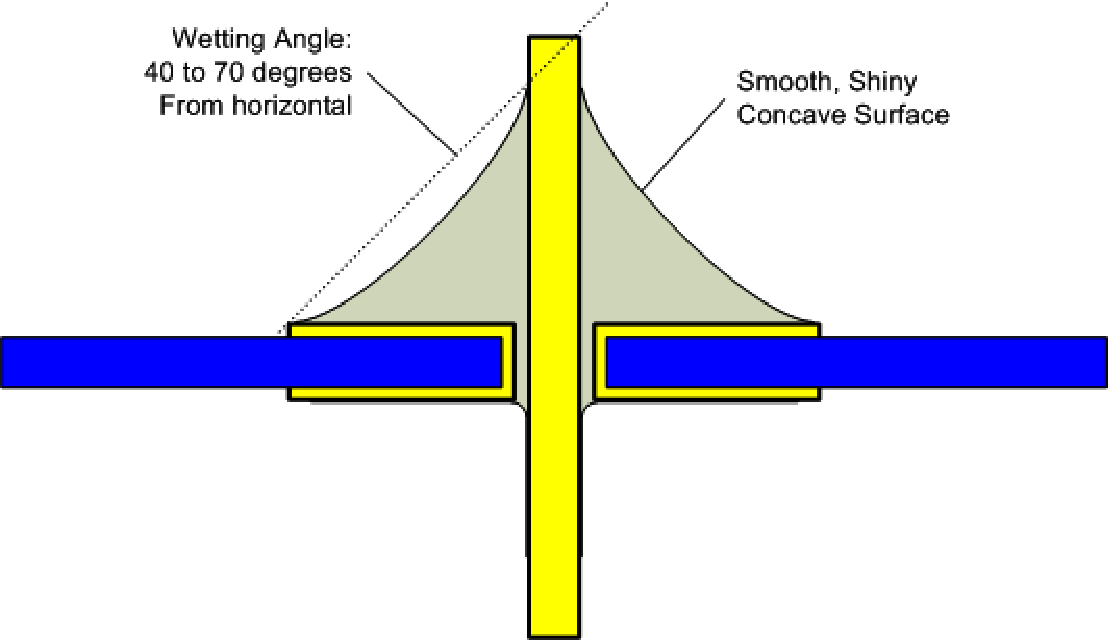
\includegraphics[width=4.5in]{images/tools_Solder_Joint.pdf}
\caption{A good solder joint. (Source: Adafruit.com)}
\label{fig:good_solder}
\end{figure}

\subsection{Tips and Tricks}
For the temperature, the iron should be set to between 343 - 371 C (650 - 700 F) for lead based solder and 371 - 400 C (700 - 750 F) for lead free solder.  Through hole and larger components will require temperatures in the upper area of these ranges while smaller components and surface mount can often use cooler temperatures.  When soldering, the solder will cool quickly and should cool to a shiny almost mirror finish.  A dull finish may indicate a poor solder connection.

When cleaning the iron, you should always have a thin coat of solder on the iron.  The point of cleaning is not to remove the solder, it is to keep the tip tinned.  Excess solder should removed when needed and when done soldering.

If the solder does not flow, the iron may be too hot and burning the tin/flux too quickly. If reducing the iron temperature does not help, you may need to use additional flux. You may also need to replace the tip or there could be a problem with the iron.  Contact a lab monitor or contact Matthew Nelson if you have any other questions or concerns with soldering.

\section{Power Supply}\label{power_supply}
The power supply is used to provide a regulated power source to a circuit under test. The power supply can also measure and record the power consumed by the circuit.

\begin{framed}
\begin{wrapfigure}{L}{0.15\textwidth}
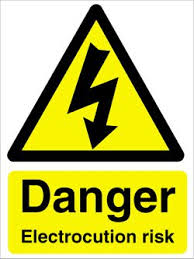
\includegraphics[width=.7in]{images/electrocution_hazard}
\end{wrapfigure}
\ \\
Both the power supplies used and your circuit may cause electrocution.  No food or drink is allowed in the electronics area and keep water usage for the sponges to a minimum.  Only energize your circuit when ready and use the over-voltage and over-current features on the power supply.
\end{framed}
\subsection{Basic Operation}
\begin{enumerate}
\item Select an appropriate channel by pushing the corresponding channel select button and wiring your circuit to the corresponding output terminals
\item Press the Voltage soft-key and program the desired output voltage using the numeric keys or the dial
\item Press the Current soft-key and program the desired output current using the numeric keys or the dial
\item Press the OVP and/or OCP soft-keys to set the desired over-voltage or over-current protection values and again to enable the protection mode
\item Turn the channel on or off by pressing the corresponding On/Off button 
\end{enumerate}

When the load voltage is higher than the programmed value, the power supply will operate in constant voltage mode and limit to the programmed voltage.  When the load current is higher than the programmed value, the power supply will operate in constant current mode and limit to the programmed current.  If the load current or voltage crosses an enabled threshold, that channel will shut down.
\subsection{Timer Operation}
Timer operation allows the user to program voltage and current steps and associated time intervals.  This may be useful for testing a range of voltages and/or current values.  To use this feature, follow these steps.

\begin{enumerate}
\item Press the Timer button to display the timer interface.
\item Press the Timer Set soft-key to set the timer parameters.
\item After setting the timer parameters, press the Timer button and then the Timer softkey to enable the timer.
\end{enumerate}

\section{Oscilloscope}
\subsection{Basic Operation}
\begin{enumerate}
\item Compensate the probe for each channel you will be using (Optional)
\begin{enumerate}
\item Set the switch on the probe to 10X.
\item Press the channel button corresponding to the channel you are using and set the attenuation factor to 10X.
\item Attach the probe lead to the compensation connector and the ground lead to the ground connector.
\item Press the Auto button and wait a few seconds.
\item A square wave will be displayed on the screen, adjust the compensation trimmer on the probe until the waveform edges are square.
\end{enumerate}
\item Attach the probe to the circuit under test.
\item Press the Auto button or adjust the vertical and horizontal div controls as desired.
\end{enumerate}
For most measurements, the probe should be left in 10X mode for the best results.

\subsection{Adjusting the Display}

\textbf{Vertical}
The vertical scale of a channel can be adjusted by pressing the channel button of interest (CH1 or CH2) and then turning the scale knob. You can switch between coarse and fine adjustment by pressing the scale knob. The current scale is displayed on the bottom line of the display. To change the vertical position on the display, turn the position knob. While adjusting the position control, a voltage is displayed, indicating the voltage offset from the ground reference. You can instantly return the offset to zero by pressing the position knob.

\textbf{Horizontal}
The horizontal time scale can be adjusted by turning the horizontal scale knob. You can move the displayed waveform left and right by turning the horizontal position knob. Pressing the position knob will instantly center the waveform. Pressing the scale knob will enable zoom mode which will allow you to inspect the waveform in greater detail.
\subsection{Performing Measurements}
\textbf{Automatic}
\begin{enumerate}
\item Press the Measure button.
\item Use the Source soft-key to select which channel the measurement is performed on.
\item Press the Voltage or Time soft-key to select the type of measurement or the Clear softkey to clear any on screen measurements.
\item Press the soft-key corresponding to the specific measurement you wish to perform. The result will be displayed on screen.
\end{enumerate}
\textbf{Cursor}
Cursor based measurements can be used to manually measure time or amplitude parameters that cannot be performed automatically.  Follow these steps to use the cursor.
\begin{enumerate}
\item Press the Cursor button.
\item Use the Mode soft-key to select the manual mode.
\item Use the Source soft-key to select which channel the measurement is performed on.
\item Use the Type soft-key to select X or Y measurements.
\item Use the A and B soft-keys and the multi-function knob to move the cursors and see the results on screen.
\end{enumerate}
\section{Waveform Generator}
\subsection{Basic Operation}
The following steps will get you started in the basics of using the waveform generator.
\begin{enumerate}
\item Press the CH1/CH2 button to select the channel of interest.
\item Press the button corresponding to the type of waveform you would like to generate.
\item Press the Freq soft-key and enter the desired frequency using the dial or number pad.
\item Press the Ampl soft-key and enter the desired amplitude using the dial or the number pad. By pressing the Ampl key a second time, you may enter the desired maximum signal level (HiLev).
\item Press the Offset soft-key and enter the desired DC offset using the dial or the number pad. By pressing the Offset key a second time, you may enter the desired minimum signal level (LoLev).
\end{enumerate}
Double check the parameters you have entered before enabling the channel output. Press the View button to change the display to a view that allows you to check the frequency and amplitude at the same time. Then press the Output button next to the channel that you are using to enable the output.
